\documentclass[12pt]{article}

\usepackage[dvips,letterpaper,margin=0.75in,bottom=0.5in]{geometry}
\usepackage{cite}
\usepackage{slashed}
\usepackage{graphicx}
\usepackage{amsmath}
\usepackage{braket}

\usepackage[american,fulldiode]{circuitikz}
\usetikzlibrary{calc}

\newcommand{\kb}{k_{\rm b}}
\begin{document}
\ctikzset{bipoles/thickness=1}
\ctikzset{bipoles/resistor/height=.115}
\ctikzset{bipoles/resistor/width=.3}
\ctikzset{bipoles/capacitor/height=.2}
\ctikzset{bipoles/capacitor/width=.06}

\title{Johnson Noise}
\author{Michael Mulhearn}

\maketitle

\section{Introduction}

Johnson--Nyquist noise is the electronic noise that results from the thermal excitation of electrons in a conductor independent of any applied voltage.  As the applied voltage is zero, there is no net potential difference due to Johnson noise ($\braket{V}=0$), but generally the average power $\braket{V^2}$ is non-zero.  As we will show, the one-sided power spectral distribution turns out to be simply:
\begin{equation}
\mathcal{S}_{+}(f) = 4 R \kb T,
\end{equation}
By measuring all of the other quantities, we will use this relation to experimentally determine Boltzman's constant, which has the value
\begin{equation*}
\kb = 1.38064852(79) \times 10^{-23} {\rm J}/{\rm K}
\end{equation*}
with the uncertainty in parenthesis.

\section{Autocorrelation and Power Spectrum Distribution}

The signal $V(t)$ associated with random noise does not have a Fourier Transform, and so the obvious mechanism for finding the frequency spectrum associated with $V(t)$ is ruled out.  Instead, we define the autocorrelation by:
\begin{equation}
\mathcal{R}(\tau) \equiv \lim_{T \to \infty } \frac{1}{T} \int_{0}^{T} dt \; V(t) V(t-\tau) = \braket{V(t) V(t-\tau)}
\label{eqn:autopower}
\end{equation}
which is part of a Fourier transform pair:
\begin{eqnarray}
\mathcal{S}(f) &\equiv& \int_{-\infty}^{\infty} d\tau \; \mathcal{R}(\tau) \exp(-i2\pi f \tau) \\ 
\mathcal{R}(\tau) &=& \int_{-\infty}^{\infty} df \; \mathcal{S}(f) \exp(i2\pi f \tau)  \label{eqn:ifts}
\end{eqnarray}
To interpret $\mathcal{S}(f)$ we note that Definition~\ref{eqn:autopower} implies that:
\begin{displaymath}
R(0) = \braket{V^2(t)} \equiv P_{\rm avg}
\end{displaymath}
but from Equation~\ref{eqn:ifts} we also have:
\begin{eqnarray*}
R(0) &=& \int_{-\infty}^{\infty} df \; \mathcal{S}(f) \exp(i2\pi f 0) \\
        &=& \int_{-\infty}^{\infty} df \; \mathcal{S}(f)
\end{eqnarray*}
or in other words:
\begin{displaymath}
P_{\rm avg} \equiv \braket{V^2(t)} = \int_{-\infty}^{\infty} df \; \mathcal{S}(f) 
\end{displaymath}
That is to say $\mathcal{S}(f)$ is the average power contained at frequency $f$.  To calculate $\mathcal{S}(f)$ we simply calculate the Fourier transform of the autocorrelation function:
\begin{equation}
\mathcal{R}(\tau) \equiv \braket{V(t) V(t-\tau)}.
\end{equation}
There are a few practical simplifications we can make resulting from the fact that $\mathcal{R}(\tau)$
is a real even function, and therefore need only calculate:
\begin{displaymath}
\mathcal{S}(f) =2  \int^{\infty}_{0} d\tau \; \mathcal{R}(\tau) \cos(2\pi f \tau).
\end{displaymath}
But now clearly $\mathcal{S}(f)$ is also an even function, and we can therefore consider the one-sided-power spectral distribution:
\begin{eqnarray}
\mathcal{S}_{+}(f) &\equiv& 2 \mathcal{S}(f) \\ 
&=& 4  \int^{\infty}_{0} d\tau \; \mathcal{R}(\tau) \cos(2\pi f \tau) 
\end{eqnarray}
which has the same interpretation as the power spectral distribution but simply restricted to positive frequencies:
\begin{equation}
P_{\rm avg} \equiv \braket{V^2(t)} = \int_{0}^{\infty} df \; \mathcal{S}_+(f) 
\end{equation}

\section{Theory of Johnson Noise}

Johnson--Nyquist noise is the electronic noise that results from the thermal excitation of electrons in a conductor independent of any applied voltage.  As the applied voltage is zero, there is no net potential difference due to Johnson noise ($\braket{V}=0$), but generally the average power $\braket{V^2}$ is non-zero.  As we will show, the one-sided power spectral distribution turns out to be simply:
\begin{equation}
\mathcal{S}_{+}(f) = 4 R k T,
\end{equation}
where the one-sided power spectral distribution $\mathcal{S}_+(f)$ is the average power per bandwidth, i.e.
\begin{displaymath}
P_{\rm avg} \equiv \braket{V^2(t)} = \int_{0}^{\infty} df \; \mathcal{S}_{+}(f) 
\end{displaymath}

Consider a resistor of resistance $R$ with no potential imposed across it.  Using the superposition principle, we'll consider that the total potential $V$ across the resistor then results from sum of the voltage caused by each individual electron due to it's current $I_i$:
\begin{displaymath}
V_i(t) = R I_i = \frac{Re}{L} u_i(t)
\end{displaymath}
where $L$ is length of the resistor and $u_i$ is the velocity along the axis of the resistor.  With no applied voltage and therefore no preferred direction we must have $\braket{u_i}=0$.  However, because each electron is in thermal equilibrium we have $m\braket{u^2_i}=kT$ and so:
\begin{displaymath}
\braket{V^2_i(t)} = R^2 \frac{e^2}{m L^2} kT.
\end{displaymath}
Assuming each electron is uncorrelated with the other electrons,
\begin{displaymath}
\braket{V_i(t) V_j(t)} = 0,
\end{displaymath}
for $i \neq j$ and so:
\begin{displaymath}
\braket{V^2(t)} =  \sum_{ij}  \braket{ V_i(t) V_j(t) } = R^2 \frac{N e^2}{m L^2} kT,
\end{displaymath}
where $N$ is the number of electrons.

The Fourier transform of $V(t)$ is not defined for continuous random noise.  However, we can still determine the power spectral distribution from the autocorrelation function, as discussed above.  In this case, the electrons are subject to collisions which alter their trajectory on a timescale $\tau_{\rm c}$, and we therefore expect the signal to become uncorrelated on that timescale:
\begin{displaymath}
\mathcal{R}(\tau) \equiv \braket{V(t) V(t-\tau)} =  A \exp(-\tau/\tau_+)
\end{displaymath} 
for $\tau \geq 0$, which is all we will need.  We note that by definition
\begin{displaymath}
\mathcal{R}(0) = \braket{V^2(t)} 
\end{displaymath}
and so we must have:
\begin{displaymath}
\mathcal{R}(\tau) = R^2 \frac{N e^2}{m L^2} kT \exp(-\tau/\tau_+).
\end{displaymath} 
With the autocorrelation function in hand, the one-sided power spectrum distribution is only an integral away:
\begin{eqnarray*}
\mathcal{S}_{+}(f) &=& 4R^2 \frac{N e^2}{m L^2} kT \int_0^{-\infty}\cos(2\pi f \tau) \exp(-\tau/\tau_{\rm c})\\
 &=& 4R^2 \frac{N e^2}{m L^2} kT \frac{\tau_{\rm c}}{1+(2 \pi f \tau_c)^2} \\
 &=& 4R kT \frac{1}{1+(2 \pi f \tau_c)^2} \\
\end{eqnarray*} 
Where in the last step we have used the fact the resistance is given by:
\begin{displaymath}
R = \frac{m L^2}{N e^2 \tau_c}.
\end{displaymath}
Noting that $\tau_c \sim 10^{-14}~\rm s$ for typical conductors, then at any frequency we are likely to encounter in an electric circuit $f \tau_c << 1$ so that the one-sided power spectral distribution is simply
\begin{equation}
\mathcal{S}_{+}(f) = 4 R k T.
\end{equation}

\section{Experimental Expectations}

We saw in the previous sections that the one-sided power spectral distribution is defined by
\begin{equation}
P_{\rm avg} \equiv \braket{V^2(t)} = \int_{0}^{\infty} df \; \mathcal{S}_+(f) 
\end{equation}
The average power is something we can easily measure.  When we measure the RMS of a signal we are measuring 
\begin{displaymath}
V_{\rm rms} = \sqrt{\braket{V^2(t)}} = \sqrt{P_{\rm avg}}
\end{displaymath}
To make a quantitative prediction for the result of this measurement, we integrate the power spectral distribution across the entire bandwidth for the circuit (all electronic circuits cut off at some high-frequency).

In the case of Johnson noise we found that:
\begin{equation}
\mathcal{S}_{+}(f) = 4 R \kb T.
\end{equation}
which is flat in frequency space.  Note that at room temperature:
\begin{displaymath}
4 \kb T =  1.6 \times 10^{-5} \frac{{\rm mV}^2}{\rm kHz M\Omega}
\end{displaymath}
so even with a $1~\rm M\Omega$ and a $10~\rm kHz$ bandwidth, the RMS voltage due to Johnson Noise will be much smaller than $1~\rm mV$.  We will need to amplify this signal with very high gain in order to see the effect of Johnson Noise.  Our gain will have a frequency dependence, even though our power spectral distribution does not, so we have:
\begin{eqnarray*}
V_{\rm rms}^2  &=& \int_{0}^{\infty} df \; g^2(f) \mathcal{S}_+(f)\\
&=& 4 \kb T R \int_{0}^{\infty} df \; g^2(f)
\end{eqnarray*}
If we approximate our circuit as having a constant gain G across a bandwidth $\Delta f$, we have:
\begin{displaymath}
V_{\rm rms}^2  = 4 \kb T R G^2 \Delta f
\end{displaymath}

The high gain devices we will be using have a bandwidth of about $10~\rm kHz$ and a fairly constant gain in the range $3000-5000$.   The devices allow you to select between resistors with values $R=1~{\rm M\Omega}, 500~{\rm k\Omega}, 100~{\rm k\Omega}, 60~{\rm k\Omega}, 30~{\rm k\Omega}$.

For a gain in the range $G=3500$ to $4000$ and $R=1~\rm M\Omega$ this would yield a power spectral density in the range of:
\begin{displaymath}
200-262~\rm mV^2/kHz
\end{displaymath}
For a $10~\rm kHz$ bandwidth, the corresponding expected RMS voltage would be $44-51~\rm mV$.

In the first week of this experiment, you will measure the gain of the Johnson Noise circuit as a function of frequency using the attenuated output from your function generator.  You will then measure the RMS voltage resulting from amplified Johnson noise and use this to determine $\kb$.

In the second week of this experiment, you will build a power spectrum analyzer, which will allow you to qualitatively investigate the (flat) Johnson noise spectrum, as well as extract $\kb$ more directly from the average PSD.

\section{Johnson Noise Device Gain Measurement}

\begin{figure}[htbp]
\begin{center}
{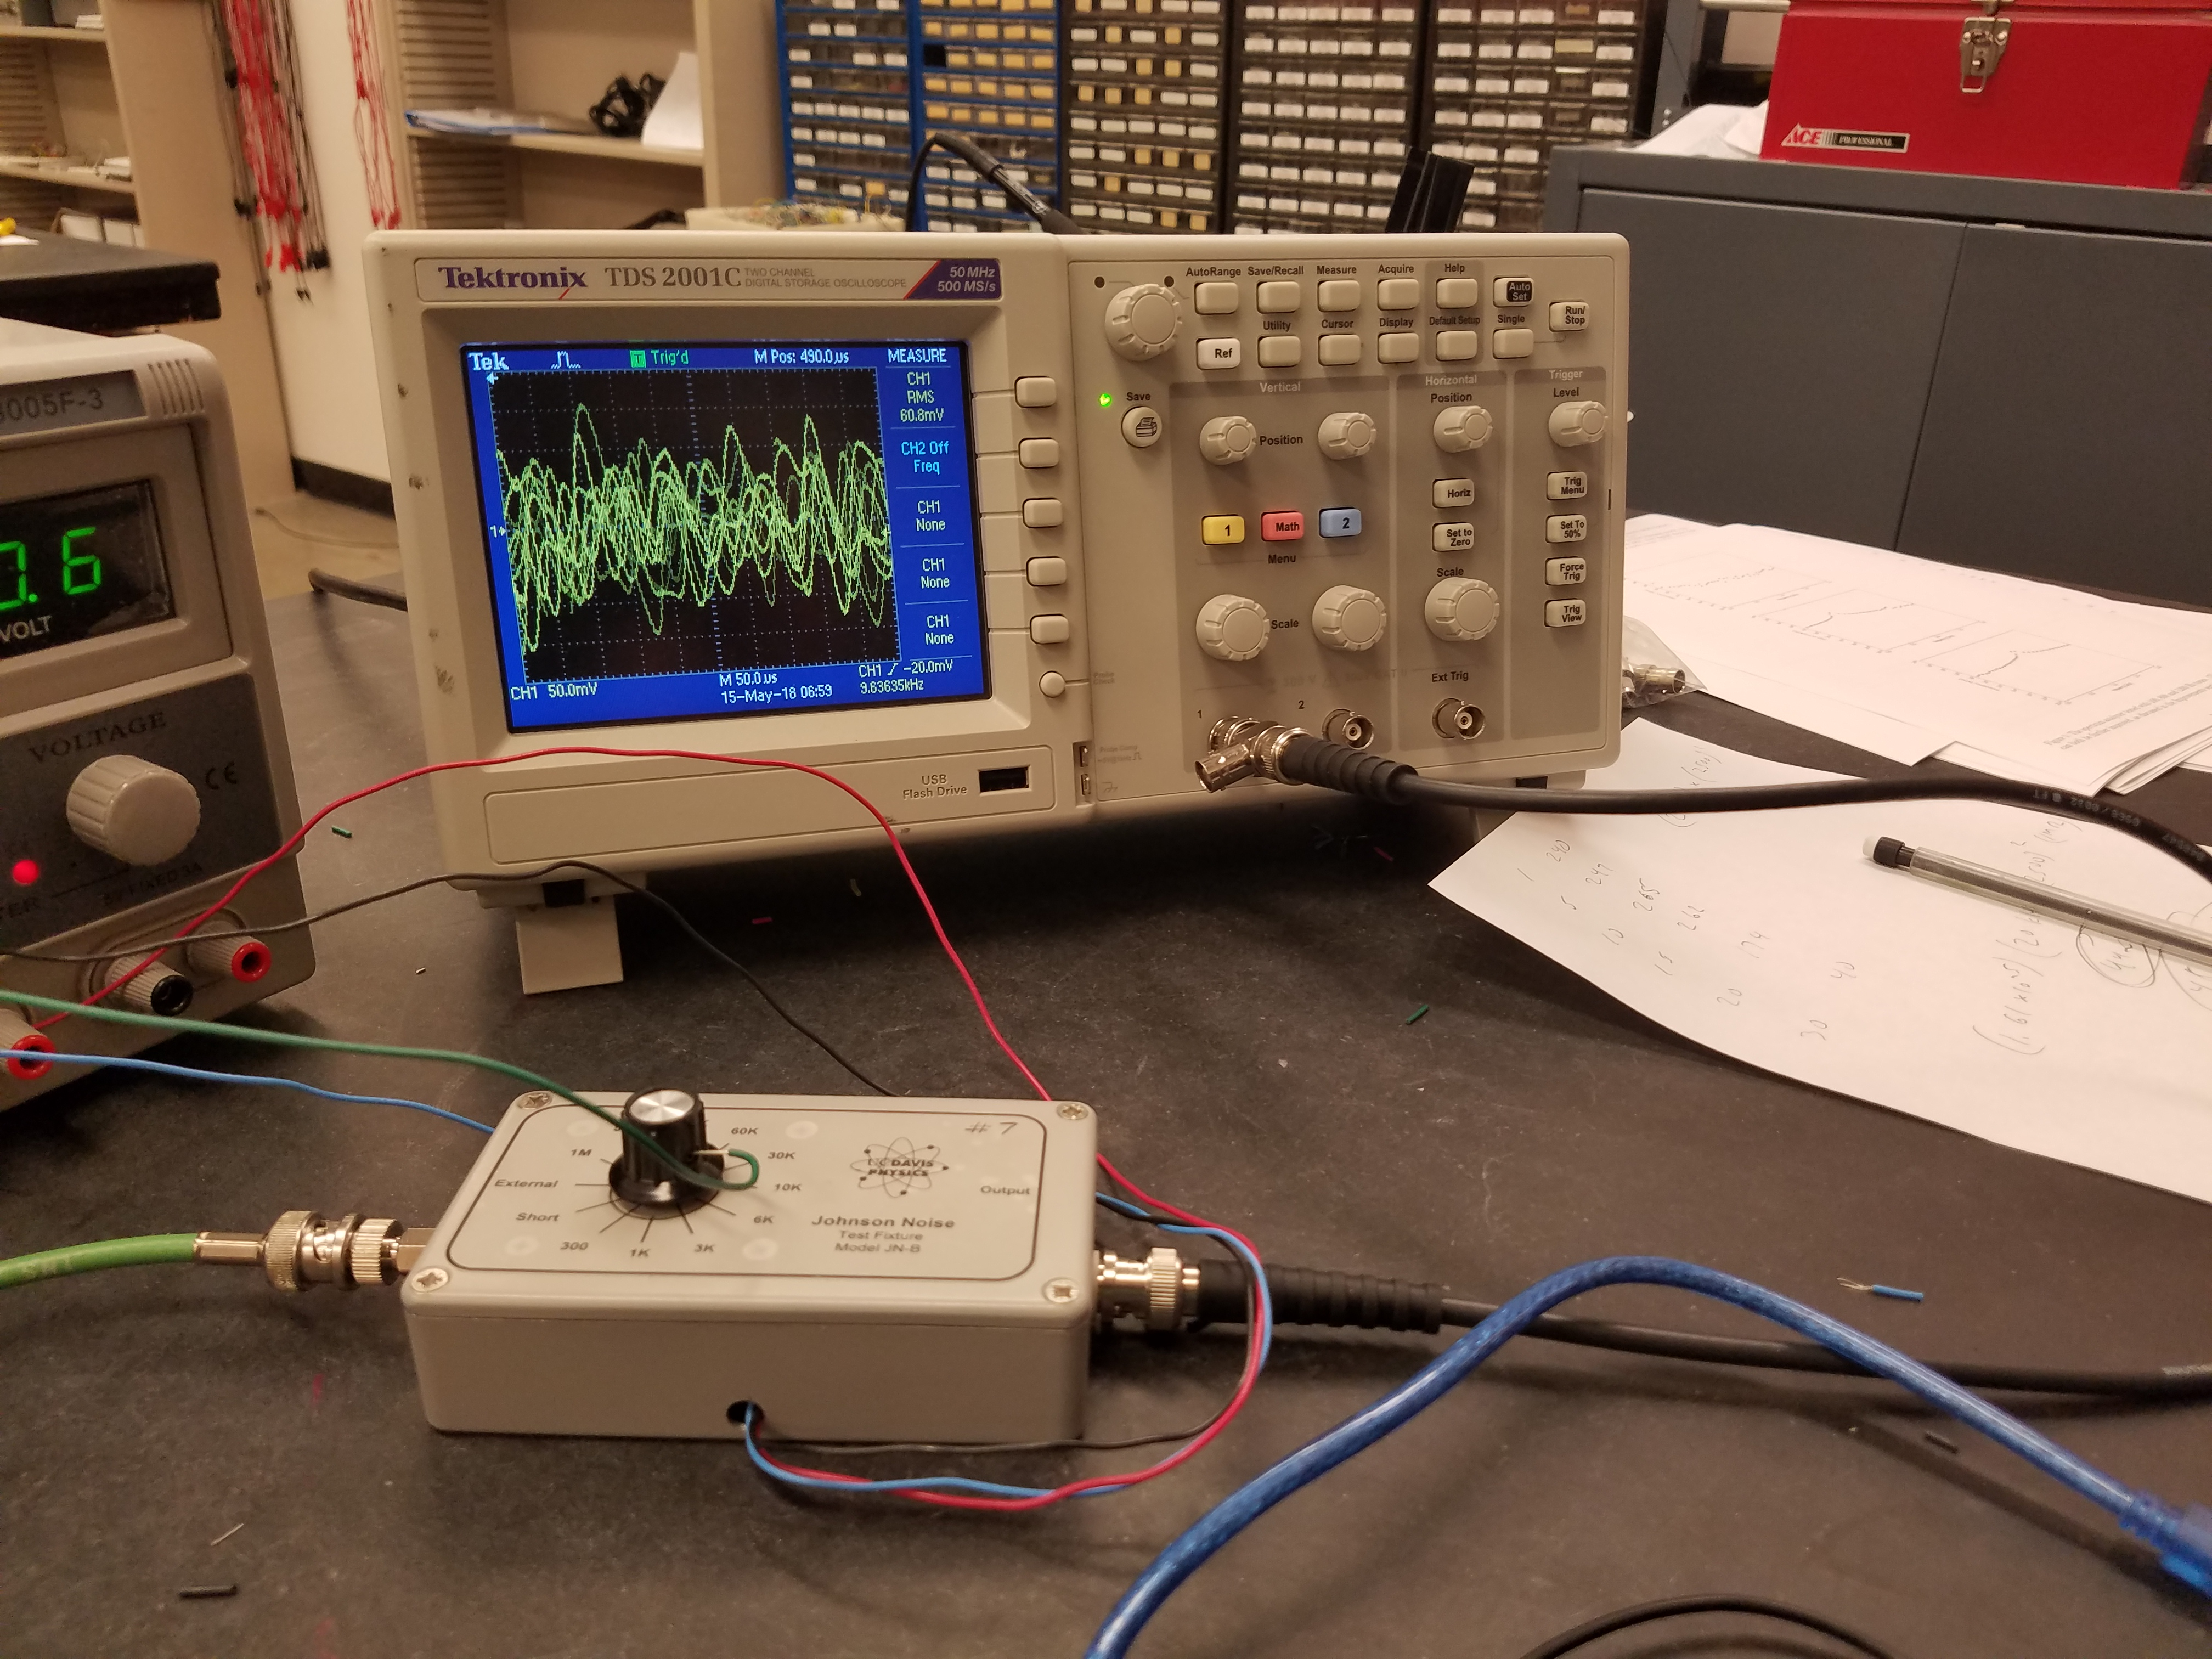
\includegraphics[width=0.65\textwidth]{figs/antenna_grounded.jpg}}
\end{center}
\caption{\label{fig:plan} Connections to the Johnson Noise device.  Note the grounding wire used to reduce noise from the knob acting as an antenna!}
\end{figure}

In this section, we will measure the gain of the Johnson Noise device as function of frequency.

Obtain a Johnson Noise (JN) measurement device (Model JN-A or JN-B) and note the serial number (e.g. \#4).  These are high gain devices that are very susceptible to damage.  Do not drive them directly from a function generator, but use a 1000:1 attenuator, taking care that the small resistor is toward the JN device (else you will reduce voltage by a factor 999/1000, and likely damage the equipment!)  

The JN devices are very sensitive, easily pickup noise, and ring at a characteristic frequency of about $27~{\rm kHz}$.  The tuning knob in particular picks up noise.  An old version banana plug cable plugged into the knob at the set screw grounds the knob, eliminated this source of noise.  The effect can be quite dramatic. 

Adjust the supply levels on your bench-top supply to $+12~{\rm V}$ and $-12~{\rm V}$.  Then, with the supply turned off, connect the JN device to power and ground, as labeled on the wires.  Once connected, power the device on and adjust the current thresholds to just slightly above where the supplies become current limited.  Under normal operation, the JN device should draw about $20~\rm mA$ from each supply... keep an eye on it.  If one of the supplies is inadvertently disconnected, the circuit latches in a high current state, which should be avoided if possible.

Set your function generator to produce a sine wave with $V_{\rm rms} = 100~\rm mV$ and $f = 1~\rm kHz$.  Connect the function generator to channel 1 of your scope, then to the $1000:1$ attenuator, and then to your JN device.  Make certain that the JN device is set to the ``External'' mode.  The output of the JN device should then be plugged directly into the scope channel 2.

\begin{figure}[htbp]
\begin{center}
{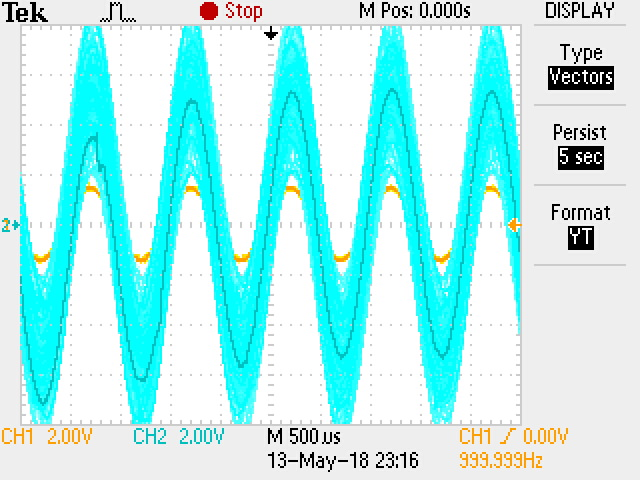
\includegraphics[width=0.65\textwidth]{figs/gaintrouble.jpg}}
\end{center}
\caption{\label{fig:gaintrouble} The output of the Johnson Noise device bounces around a lot due to low frequency noise.  Here the output is shown with display persistance.}
\end{figure}

Make a series of gain measurements at different frequencies that will allow to determine the integral
\begin{displaymath}
\int_{-\infty}^{\infty} df g(f)^2.
\end{displaymath}
While making the gain measurement, you will see that the output of the Johnson Noise seems to bounce around.  The effect can be seen if Fig.~\ref{fig:gaintrouble}.  There is a significant amount of low frequency noise in the output.  I found the best approach was to trigger on the AC line, which allows you to find a region of the plot with relatively little 60 Hz noise.  Use the scopes Measure capability to find the RMS voltage of the input and output of the Johnson Noise.  This is likely the major systematic uncertainty in your measurement, so spend some time thinking about how to quantify it. 

You might be tempted to try and use your DMM to measure the RMS voltage of your signal, but this is a mistake.  Your DMM is designed to measure 60~\rm Hz AC.

\section{Johnson Noise Measurement}
You are now ready to make your first-pass Johnson Noise measurement:
\begin{itemize}
\item Turn down the function generator and disconnect it from the JN device.

\item Turn the knob to select a resistor, and note the RMS voltage from the scope.  Repeat this measurement for every resistance.  
\end{itemize}

These measurements, combined with the gain measurement, should allow you to calculate $\kb$.
Before leaving, do make certain that the data you have collected is reasonable.  At this stage, within an order of magnitude of $\kb$ is acceptable.  {\bf This is the end point for week one.}  

\section{Digital Dynamic Range Adjustment}

In the second week of the lab, you will build a digital spectrum analyzer based on the Arduino Uno.
The Arduino's analog inputs have an input voltage range from 0 to 5 V, but our signals are ground referenced (symmetric about $0~\rm V$).  A DC level shifter is therefore needed to map the ground referenced output of the Johnson Noise device to the $0$ to $5~\rm V$ range expected by the Arduino analog inputs.  

Of course we'll be running the ADC as fast as possible which comes at the price of reduced resolution to 8 bits.  That would result in a voltage precision of $5~\rm V/ 2^8 \sim 20~\rm mV$.  Considering we will be looking at $\sim 100~\rm mV$ signals, this is just not enough precision.  Fortunately, we have one last trick up our sleeve!  The ADC has an (optional) external voltage reference, which sets the scale used by the ADC.  Experimentation showed that the ADC works reliably down to a voltage reference of $\sim 780~\rm mV$, which, at 8-bit precision, would give us a $3~\rm mv$ voltage precision, plenty good enough!

The low-pass filter in Fig.~\ref{fig:pwm} is used to convert PWM output (on pin 5 of the Arduino) into a DC reference voltage $V_{\rm ref}$.  This reference voltage is used as (1) the reference for the ADC, at pin AREF, setting the dynamic range of the ADC, and (2) the reference to the DC level shifter circuit in Fig.~\ref{fig:offset} so that input to the ADC is referenced to $V_{\rm ref}/2$.  In this way, we can adjust $V_{\rm ref}$ to match the dynamic range of our signal, and the DC offset will be set to the middle of this range.  This will ensure that even for small signals, the full 8-bit precision of the ADC is being put to use.

\begin{figure}[htbp]
\begin{center}
\begin{circuitikz}[line width=1pt]
\draw (0,0) node[ground]{} to[pC,l=$C_1$,/tikz/circuitikz/bipoles/length=0.6cm] ++(0,1.5) coordinate(X);
\draw (X) to[R,l=$R_5$] ++(0,1.5) to[short,-o] ++ (-1.0,0) node[left]{$(5) \to V_{\rm pwm}$};
\draw (X) to[short,*-o] ++(1.0,0) node[right]{$V_{\rm ref} \to ({\rm AREF}) $};
\end{circuitikz} 
\end{center}
\caption{\label{fig:pwm} A low pass filter used to convert the Arduino PWM output (on pin 5) to an analog DC reference voltage (sent to pin AREF and also used by the DC level shifter.)}
\end{figure}

\begin{figure}[htbp]
\begin{center}
\begin{circuitikz}[line width=1pt]
\draw (0,0) node[op amp, yscale=-1](opamp){}; 
\draw (opamp.-) to[short] ++(0.0,-1.0) coordinate(X) to[short] ++(1.0,0) to[R,l=$R_4$] ++(1.0,0) -| (opamp.out);
\draw (opamp.out) to[short,-o] ++(0.5,0) node[right]{$V_{\rm out} \to \rm (A0)$};
\draw (X) to[R,l_=$R_3$] ++(-1.5,0) node[ground]{};
\draw (opamp.+) to[short] ++(0,0.5) to[R,l_=$R_1$] ++(-1.5,0) to[short,-o] ++(0,0) node[left]{$V_{\rm in}$};
\draw (opamp.+) to[short] ++(0,-0.5) to[R,l_=$R_2$] ++(-1.5,0) to[short,-o] ++(0,0) node[left]{$({\rm AREF}) \to V_{\rm ref} $};
\end{circuitikz} 
\end{center}
\caption{\label{fig:offset} A DC level-shifter with unit gain.  The points (AREF) and (A0) refer to the Arduino pins, which should be connected as shown.}
\end{figure}

\begin{figure}[htbp]
\begin{center}
{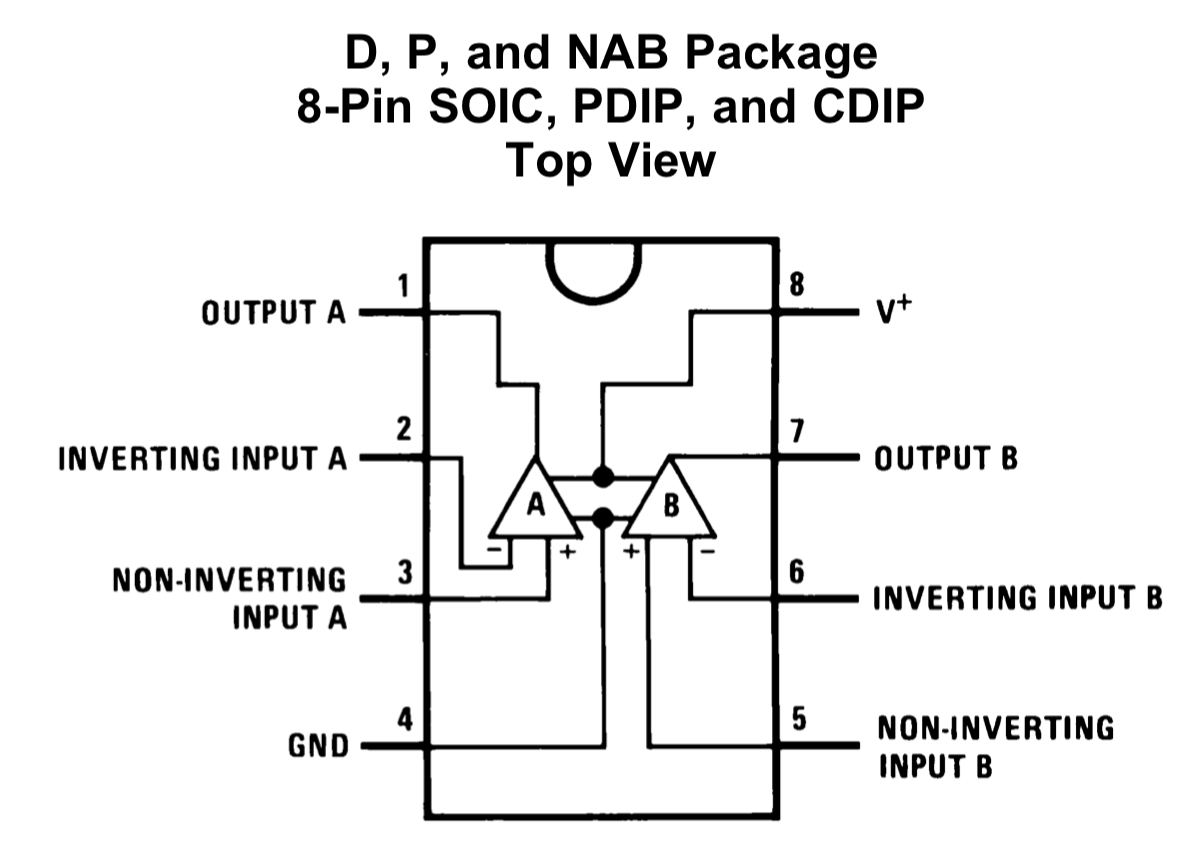
\includegraphics[width=0.65\textwidth]{figs/lm358.png}}
\end{center}
\caption{\label{fig:lm358} Pinout for the LM358 dual-op-amp with single-ended supply.  We'll only need one of the op-amps.}
\end{figure}

For our op-amp we will use a LM358 low-power dual op-amp IC with pinout in Fig.~\ref{fig:lm358}.
The LM358 is designed to run off a single supply down to $5~\rm V$, so we can power this circuit entirely from the Arduino.  This is not just convenient, it also ensures that it's output cannot exceed the $0$ to $5~\rm V$ range expected by the Arduino.

You will build the circuits in Fig.~\ref{fig:pwm}  and \ref{fig:offset} using $R_1 = R_4 = 33~\rm k\Omega$, $R_2 = R_3 = 15~\rm k\Omega$, $R_5=1~k\Omega$.  For $C_1$ use a large polarized capacitor ($C_1=330~\rm  \mu F$) and {\bf make certain that the negative terminal is connected (as shown in the circuit) to ground.}  Connect the positive supply of the Op Amp to the $5~V$ supply of the Arduino and the $0~V$ supply to the Arduino ground.  

A light-weight sketch {\rm CircuitTester} is provided which is useful while developing your circuit.  This sketch implements an RMS voltmeter (significantly better, if less durable, than the one provided by your DMM.) based on the circuit your are building.  It provides control of the PWM on pin 5, reads the analog input on A0, and regularly reports the RMS voltage (and other useful quantities) on the serial output.
The level of the PWM is specified in the parameter {\rm RUN\_SCALE}.  A value of 0 results in $0\%$ duty-cycle for the PWM, a value of 255 corresponds to $100\%$ duty-cycle.

While testing your circuit, you should use your function generator to drive the input $V_{\rm in}$ directly.  A $5~\rm kHz$ sine function with an RMS amplitude of $100~\rm mV$ is a good starting point.  Make sure the ground of the function generator is connected to the ground of your Arduino.

By now we've learned to divide and conquer technical challenges!  I'd propose something like:
\begin{itemize}
\item Leave the Arduino unpowered.
\item Build the level shifter as shown but at first (1) set the reference voltage to $5~\rm V$ and (2) connect the output to channel one on your scope instead of pin A0.
\item Power up the Arduino.
\item On your scope you should see the function generator referenced to approximately $2.5~\rm V$.
\item Power down the Arduino.
\item Build the lowpass filter as shown, but  connect $V_{\rm ref}$ to channel two on our scope instead of to pin {\tt AREF}.
\item Power up the Arduino and download the {\rm CircuitTester} sketch, setting the parameter {\tt RUN\_SCALE} to 112.
\item On your scope, you should observe $V_{\rm ref}$, it should be at about $2.5~\rm V$ with very little ripple (use AC line trigger and DC offset).
\item Adjust the {\tt RUN\_SCALE} parameter and ensure you have the expected behavior.
\item Power down the Arduino.
\item Connect the lowpass filter output $V_{\rm ref}$ to both $({\rm AREF})$ and the DC level-shifter input $V_{\rm ref}$.
\item Power up the Arduino.
\item Check that level-shifter output has the correct DC level when you adjust {\tt RUN\_SCALE}.
\item Connect the output of the DC level-shifter to the Arduino analog input A0.
\item Start the Serial Monitor.
\end{itemize}

Once the whole circuit is built, the Arduino is running the {\tt CircuitTester} sketch, and the Serial Monitor is open, you should observe periodic RMS voltage readings that should correspond approximately with the output of the function generator.

\section{Calibration of Arduino Circuit}

\section{Improved Johnson Noise Device Gain Measurement}


\section{Johnson Noise Measurement}


\end{document}


